\section{Einleitung}

Ziel dieses Versuchs ist der Aufbau und die Kontrastmessung eines Sagnac-Interferometers, sowie die Bestimmung der Brechungsindices von Luft in Abhängigkeit des Luftdrucks und Glas mit eben diesem Interferometer.

\section{Theorie}

Im Folgenden soll zuerst die Entstehung von Interferenzeffekten erläutert werden \cite{Lit1}.
Die Wellencharakteristik von elektromagnetischer Strahlung kann durch
\begin{equation*}
  \vec{E}(\vec{r},t) = \vec{E_0} \cdot e^{i(\omega t - \vec{k}\vec{r})}
\end{equation*}
beschrieben werden.
Dabei ist $\vec{k}$ der Wellenvektor der Strahlung, $\omega$ ihre Frequenz und $\vec{E_0}$ die Amplitude.
Bei kohärentem Licht und gleicher Polarisationsrichtung kommt es bei Überlagerung zur Interferenz.
Für zwei interferierende Wellen
\begin{align*}
  \vec{E_1}(\vec{r},t) &= \vec{E_{1,0}} \cdot e^{i(\omega t - \vec{k}\vec{r})} \, , \\
  \vec{E_2}(\vec{r},t) &= \vec{E_{2,0}} \cdot e^{i(\omega t - \vec{k}\vec{r} + \gamma)} \, ,
\end{align*}
wobei $\vec{E_2}$ eine Phasenverschiebung $\gamma$ zu $\vec{E_1}$ aufweist, folgt für die Intensität
\begin{equation}
  I = \Bigl \langle |\vec{E_1} - \vec{E_2}|^2 \Bigr \rangle = E_{1,0} + E_{2,0} + 2 E_{1,0} E_{2,0} \cos(\gamma) \, .
  \label{eqn:Intensität}
\end{equation}
Für gleiche Amplituden $E_{1,0} = E_{2,0} = E$ folgt für die Intensität
\begin{equation}  \label{eqn:Gl2}
  \begin{aligned}
  \gamma &= \pi &\rightarrow& &I_\text{min.} &= 0 \, , \\
  \gamma &= 0 &\rightarrow& &I_\text{max.} &= 4E \, .
\end{aligned}
\end{equation}

\bigskip

Bislang wurden nur Wellen mit gleicher Polarisation und Polarisationsrichtung betrachtet.

Das Herzstück des Sagnac-Interferometers bildet jedoch ein \textit{Polarizing Beam Splitter Cube} (PBSC).
\begin{wrapfigure}[15]{r}{.4\textwidth}
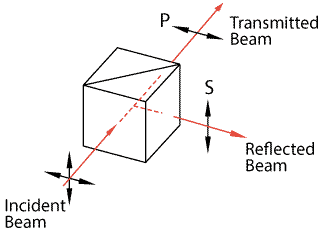
\includegraphics[width = .3\textwidth]{bilder/sketch-polarizing-cube-beamsplitter.png}
\caption{Schematische Zeichnung eines PBSC und die Polarisationsrichtungen des Lichts \cite{PBSC}.}
\label{fig:PBSC}
\end{wrapfigure}
Dieser transmittiert Licht, welches parallel zur horizontalen Achse des PBSC polarisiert ist und reflektiert Licht, welches vertikal polarisiert ist (vlg. Abbildung \ref{fig:PBSC}).
Daher muss für die weitere Betrachtung die Polarisationsrichtung des, auf den PBSC treffenden, Lichtes beachtet werden.
Linear polarisiertes Licht $E$, dessen Polarisationsrichtung den Winkel $\phi$ zur horizontalen Achse des PBSC aufweist, wird durch diesen in den transmittieren Anteil
\begin{equation*}
  E_{\_} = E \cos(\phi)
\end{equation*}
und den reflektierten Anteil
\begin{equation*}
  E_{\bot} = E \sin(\phi)
\end{equation*}
aufgeteilt.
\medskip
Bei Interferenz dieser beiden Strahlen ergibt sich nach Gleichung \eqref{eqn:Intensität} für die Intensität der Interferenz
\begin{equation*}
  I = E^2 \cdot (1 + 2 \cos(\phi) \sin(\phi) \cos(\gamma))
\end{equation*}
aus dieser folgt für die Phasenverschiebung analog zu \eqref{eqn:Gl2}
\begin{equation}  \label{eqn:Gl3}
  \begin{aligned}
  \gamma &= \pi &\rightarrow& &I_\text{min.} &= E^2 \cdot (1 − \sin(2\phi) \, , \\
  \gamma &= 0 &\rightarrow& &I_\text{max.} &= E^2 \cdot (1 + \sin(2\phi) \, .
\end{aligned}
\end{equation}

Eine wichtige Kenngröße eines Sagnac Interferometers ist sein Kontrast
\begin{equation}
  K = \frac{I_\text{max.} - I_\text{min.}}{I_\text{max.} + I_\text{min.}} = \sin(2\phi) \, .
  \label{eqn:Kontrast}
\end{equation}
Es wird schnell ersichtlich, dass dieser bei einer Polarisationsrichtung von $\phi = \SI{45}{\degree}$ maximal ist, da $\cos(\SI{45}{\degree}) = \sin(\SI{45}{\degree})$ und damit der reflektierte Anteil des eingestrahlten Lichtes genauso groß ist, wie der transmitierte Anteil.


\subsection{Brechungsindex von Glas}
Fällt Licht im Winkel $\delta$ auf eine planparallele Glasplatte, beträgt die Phasenverschiebung $\Delta \gamma$ nach \cite{anleitung} für kleine Winkel $\delta$
\begin{equation} \label{eqn:Phasendifferenz}
  \Delta \gamma = \frac{2 \pi}{\lambda_\text{vac.}} \, T \, \frac{n-1}{2n} \delta^2 \, .
\end{equation}
Die Phasenverschiebung ist somit abhängig von der Wellenlänge $\lambda_\text{vac.}$ des Lichts im Vakuum, der Dicke $T$ der Glasplatte und dem Brechungsindex $n$ des Glases.
Durch Veränderung des Winkels $\delta$ können also Phasendifferenzen erzeugt werden, die zu Interferenzeffekten mit Licht führen, welches keine Glasplatte passiert hat.
Aus der Anzahl $M = \sfrac{\Delta \gamma}{2 \pi}$ der Phasenverschiebungen um \SI{360}{\degree} bei Drehung der Glasplatte um den Winkel $\delta$ kann nach Umstellen der Gleichung \eqref{eqn:Phasendifferenz} der Brechungsindex
\begin{equation}\label{eqn:n_Glas}
  n = \left( 1 - \frac{2 M \lambda_\text{vac.}}{T \delta^2} \right)^{-1}
\end{equation}
berechnet werden.


\subsection{Brechungsindex von Gas}

Wird der Lichtstrahl durch einen mit Gas gefüllten Raum der Länge $L$ geleitet, folgt
\begin{equation} \label{eqn:n_Gas}
  \begin{split}
  \Delta \gamma &= \frac{2 \pi}{\lambda_\text{vac.}} \, (n-1) \, L \\
  \leftrightarrow n &= \frac{\lambda_\text{vac.}}{L} \,  M + 1
  \end{split}
\end{equation}
Es ist also möglich aus einer gemessenen Anzahl $M$ an $2 \pi$ Phasenverschiebungen den Brechungsindex $n$ des Gases zu bestimmen.
Weiterhin kann aus einer solchen Messung in Abhängigkeit des Drucks $p$ durch
\begin{equation*}
  n = \frac{\Delta n}{\Delta p} \, p + n_{p=0}
\end{equation*}
der Brechungsindex eines Gases für beliebige Drücke abgeschätzt werden.
